%**
%*  @file  deltacloud.tex
%*  @brief   DIET usage with cloud middlewares via deltacloud
%*  @author  - Lamiel Toch (lamiel.toch@ens-lyon.fr)
%*  @section Licence 
%*    |LICENSE|


\chapter{DIETCloud via Deltacloud}\label{chapter:Deltacloud}




\section{SeDCloud}

\subsection{Introduction}

A \emph{SeDCloud} is a SeD which offers functionnalities to interact with
different cloud middlewares. It relies on the Deltacloud
layer~\cite{Deltacloud}.  A SeDCloud acts as a client which sends
request to the Deltacloud server thanks to the C/C++ libdeltacloud
API. This API is available in the git repository : \texttt{git clone
  git://git.fedorahosted.org/deltacloud/libdeltacloud.git}.
This version of DIET was tested with the libdeltacloud version 0.9.

\subsection{Overview of the SeDCloud class}

The SeDCloud class encapsulates the standard mechanism of DIET server.
As a SeDCloud is a DIET server, this class was designed to be a
singleton. So in a server up to one SeDCloud instance can be created.
A SeDCloud instance is created by invoking the static method :
\texttt{SeDCloud::create(\ldots)}.  The only SeDCloud instance can be
obtained with the static method \texttt{SeDCloud::get()}.  In order to
launch the DIET server, the static method \texttt{SeDCloud::launch()}
must be called.

\subsubsection{DIET services linked to binaries inside VMs}

The SeDCloud instance may rely on VMs to execute remotely softwares and
retrieve results from VMs. To define such a service which execute
softwares in VMs the method \texttt{service\_table\_add()} can be used
before launching the SeDCloud (SeDCloud::launch()).

We define as ``binary'' a directory which contains executable files
and data. A binary has an entry point which is an executable file.  A
functionnality of the SeDCloud consists of copying a binary linked to
a DIET service, into Virtual Machines. Nevertheless, a binary can
already be preinstalled in Virtual Machines in which case no copy of
the binary is required. 

The method is defined as follows:

\begin{verbatim}
  int SeDCloud::service_table_add(
         const std::string& name_of_service,
         int last_in,
         int last_out,
         const diet_convertor_t* const cvt,
         const std::string& local_path_of_binary,
         const std::string& remote_path_of_binary,
         const std::string& entryPoint = "exec.sh",
         const std::string& remote_path_of_arguments = "",
         ArgumentsTransferMethod argumentsTransferMethod = filesTransferMethod,
         dietcloud_callback_t prepocessing = NULL,
         dietcloud_callback_t postprocessing = NULL)
\end{verbatim}

In fact, the method \texttt{service\_table\_add()} makes an internal
call to the classical\\ \texttt{diet\_service\_table\_add} ; among
others, it takes as parameters, the name of the service, the index of
the last input, the index of the last output. All arguments of the
service are either \texttt{DIET\_FILE} or
\texttt{DIET\_STRING}. Currently mixture of \texttt{DIET\_FILE} and
\texttt{DIET\_STRING} arguments is not implemented yet. DIET client
can invoke \texttt{diet\_call} with either \texttt{DIET\_FILE} for
input and ouput arguments, in which case files are transfered between
the SeDCloud and the VMs, or he can use \texttt{DIET\_STRING} for the
path of files passed in arguments. Note that in case where DIET client
uses \texttt{DIET\_STRING} for arguments, all files must be accessible
to the Virtual Machine which need them: a simple way is to use a NFS
server reachable from all Virtual Machines. Now, we describe the other
parameters specific to the method.
\texttt{SeDCloud::service\_table\_add()}:
 \begin{itemize}
   \item \texttt{local\_path\_of\_binary}: the local path of the
     binary (folder) in the SeDCloud machine. If
     \texttt{local\_path\_of\_binary} is set to \texttt{""} it means
     that the service is linked to a preinstalled binary inside the
     Virtual Machines.
   \item \texttt{remote\_path\_of\_binary}: the absolute path of the
     destination folder which will contains the binary files (or which
     already contains the binary files)
   \item \texttt{entryPoint}: the file which is the entry point of the
     software which is linked to the service
   \item \texttt{remote\_path\_of\_arguments} is the folder which will
     receive the input file arguments, in case where arguments are
     \texttt{DIET\_FILE}.  \texttt{remote\_path\_of\_arguments} is
     ignored in case where arguments are \texttt{DIET\_STRING}.
   \item \texttt{argumentsTransferMethod} is either
     \texttt{filesTransferMethod} in which case, the arguments of the
     service expect \texttt{DIET\_FILE} or
     \texttt{pathsTransferMethod} in which case, the service's
     arguments are expected to be \texttt{DIET\_STRING}.
     \texttt{preprocessing} and \texttt{postprocessing} are pointers
     to functions with the shape \texttt{int (*
       myFunction)(diet\_profile\_t*)}. \texttt{preprocessing} is
     called before executing remote software, and
     \texttt{postprocessing} is called after.
 \end{itemize}


Since the SeDCloud perform a ``rsync'' to copy binaries, do not forget
$/$ - which means a copy of the contents of the folder- at the end of
the local binary folder path and give absolute path to the
destination.

\subsubsection{Installing binaries inside VMs with Puppet}



\subsection{Overview of different behaviours of SeDCloud\label{sec:SeDCloudActions}}



The \texttt{SeDCloudActions} class allows to modify the behaviour of a
SeDCloud instance. To use a SeDCloud instance, a pointer to an
instance of \texttt{SeDCloudActions} must be passed to the static
method : \texttt{SeDCloud::create(SeDCloudActions*)}. A behaviour
consists of some actions:

\begin{itemize}
  \item perform\_action\_on\_sed\_creation: action performed as soon as the SeDCloud is instanciated
  \item perform\_action\_after\_service\_table\_add: action performed when the SeD developper adds a service to the SeDCloud
  \item perform\_action\_on\_sed\_launch: action performed as soon as the SeD is launched
  \item perform\_action\_on\_begin\_solve: action performed just before a problem is solved
  \item perform\_action\_on\_end\_solve: action performed just after a problem is solved
  \item when the SeD is destroyed: action performed as soon as the
    administrator presses the combination \texttt{Ctrl + C} on his keyboard to stop the SeD
\end{itemize}
Five classes which inherit from \texttt{SeDCloudActions} class are predefined.


\begin{itemize}
  \item \textbf{SeDCloudAndVMLaunchedActions}:
    \begin{enumerate}
      \item perform\_action\_on\_sed\_creation: \textbf{instanciation of VMs}
      \item perform\_action\_after\_service\_table\_add: \textbf{no action}
      \item perform\_action\_on\_sed\_launch: \textbf{copy binaries into all VMs}
      \item perform\_action\_on\_begin\_solve: \textbf{no action}
      \item perform\_action\_on\_end\_solve: \textbf{no action}
      \item when the SeD is destroyed (\texttt{Ctrl + C}): \textbf{destruction of VMs}
    \end{enumerate}
 
  \item \textbf{SeDCloudVMLaunchedAtFirstSolveActions}:
    \begin{enumerate}
        \item perform\_action\_on\_sed\_creation: \textbf{no action}
        \item perform\_action\_after\_service\_table\_add: \textbf{no action}
        \item perform\_action\_on\_sed\_launch: \textbf{record service names}
        \item perform\_action\_on\_begin\_solve: \textbf{if number of calls to solve is equal to 1 then instanciation of VMs and copy all binaries into all VMs}
        \item perform\_action\_on\_end\_solve: \textbf{no action}
        \item when the SeD is destroyed (\texttt{Ctrl + C}):
          \textbf{destruction of VMs if there are any}
      \end{enumerate}
  \item \textbf{SeDCloudVMLaunchedAtSolveThenDestroyedActions}:
    \begin{enumerate}
        \item perform\_action\_on\_sed\_creation: \textbf{no action}
        \item perform\_action\_after\_service\_table\_add: \textbf{no action}
        \item perform\_action\_on\_sed\_launch: \textbf{record service names}
        \item perform\_action\_on\_begin\_solve: \textbf{instanciation of VMs and copy the corresponding binary into all VMs}
        \item perform\_action\_on\_end\_solve: \textbf{destruction of VMs}
        \item when the SeD is destroyed (\texttt{Ctrl + C}): \textbf{no action}
      \end{enumerate}
  \item \textbf{SeDCloudMachinesActions}:
    \begin{enumerate}
        \item perform\_action\_on\_sed\_creation: \textbf{no action}
        \item perform\_action\_after\_service\_table\_add: \textbf{no action}
        \item perform\_action\_on\_sed\_launch: \textbf{copy binaries into all Machines}
        \item perform\_action\_on\_begin\_solve: \textbf{no action}
        \item perform\_action\_on\_end\_solve: \textbf{no action}
        \item when the SeD is destroyed (\texttt{Ctrl + C}): \textbf{no action}
   \end{enumerate}

  \item \textbf{SedCloudActionsNULL}:
    \begin{enumerate}
        \item perform\_action\_on\_sed\_creation: \textbf{no action}
        \item perform\_action\_after\_service\_table\_add: \textbf{no action}
        \item perform\_action\_on\_sed\_launch: \textbf{no action}
        \item perform\_action\_on\_begin\_solve: \textbf{no action}
        \item perform\_action\_on\_end\_solve: \textbf{no action}
        \item when the SeD is destroyed (\texttt{Ctrl + C}): \textbf{no action}
   \end{enumerate}
\end{itemize}

N.B.: When $n$ Virtual Machines are instanciated, a Master VM is
arbitrarily choosen and a file containing the $n$ ip addresses of VMs
is send to it. This file is in a text format where each line is one ip
address.



\section{Configuration of compilation}

\subsection{Requirements}

In order to enable the compilation and installation of the DIETCloud
with Deltacloud support, you must enable the DIET\_USE\_DELTACLOUD
flag. You also must have installed libdeltacloud.

\subsection{Warnings}

The library libdeltacloud depends on libcurl. If you use libcurl
installed out of the box on your linux system, you may encounter a known bug
in relationship with a synchronous DNS lookup. In order to work around
this bug, you can compile libcurl with \emph{ares} support. You can find more
information at this page
\url{http://curl.haxx.se/dev/readme-ares.html} about the procedure.

\subsection{Examples of clients/servers}

In order to enable the compilation and installation of examples
showing the principles of the DIETCloud with Deltacloud support, you
must enable the DIET\_BUILD\_EXAMPLES flag. Sources of the examples
can be found in : $<$diet\_src$>$/src/examples/delta-cloud.


\section{List of services}

A SeDCloud offers a predefined set of service which can be registered
thanks to methods with the shape service\_XXXX\_add().

\subsection{Instanciation of Virtual Machines}

The main important service offered by a SeDCloud is the instanciation
of Virtual Machines. This service is registered by the method
\texttt{service\_homogeneous\_vm\_instanciation\_add(const
  CloudAPIConnection&)} of the only instance of the class
\texttt{SeDCloud}. \texttt{CloudAPIConnection} is a class which stores
credentials of the user of the cloud middleware linked to
Deltacloud. The constructor of this class takes respectively as
parameters, firstly, the exposed url of the Deltacloud server (e.g.
\url{http://localhost:3001/api}), secondly, the name of the user of
cloud middleware and finally, his password. In order to make a cloud
federation, the administrator of the SeDClouds should launch serveral
instance of Deltacloud, each of them connected to a cloud
middleware. Figure~\ref{fig:SeDCloudVMInstanciator} shows a example of
such a deployment of SeDClouds which act as VM instanciators.  Each
SeDCloud knows the url of the Deltacloud server that it is linked
to. Table~\ref{tab:homogeneous-vm-instanciation} shows the DIET
profile of this service whose path is
``homogeneous\_vm\_instanciation''.

\begin{figure}[h!]
 \begin{center}
 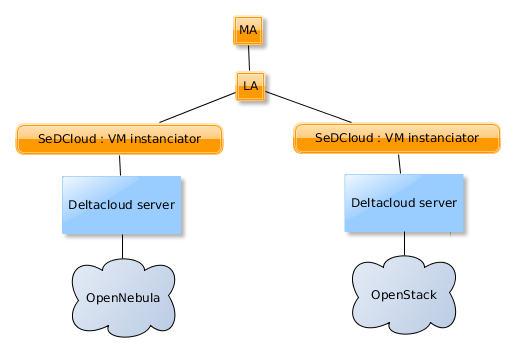
\includegraphics[width=0.7\textwidth]{fig/SeDCloudVMInstanciator}
  \caption{VMs instanciators over a federation of clouds}
  \label{fig:SeDCloudVMInstanciator}
 \end{center}
\end{figure}

\begin{table}[h!]
\begin{tabular}{|c|c|c|p{0.5\textwidth}|} 
  \hline
  \multicolumn{4}{|c|}{Service name : \textbf{\texttt{homogeneous\_vm\_instanciation}}} \\
  \hline
    IN/OUT & Position & Type & Description \\
    \hline
    \multirow{5}{*}{IN} & 0 & DIET\_INT & Number of VMs to instanciate\\
    \cline{2-4}
                        & 1 & DIET\_STRING & Image's id of the VMs to instanciate\\
    \cline{2-4}
                        & 2 & DIET\_STRING & VM's profile\\
    \cline{2-4}
                        & 3 & DIET\_STRING & User login of the VMs\\
    \cline{2-4}
                        & 4 & DIET\_INT & If 0 then the ip addresses of the VMs are considered by Deltacloud as public ip, private ip otherwise\\
    \hline
    \multirow{1}{*}{OUT} & 5 & DIET\_FILE & A file containing ip addresses of VMs \\
    \hline
\end{tabular}
\caption{DIET profile of the service ``homogeneous\_vm\_instanciation''}
\label{tab:homogeneous-vm-instanciation}
\end{table}



\subsection{Destruction of Virtual Machines}

A SeDCloud can destroy a set of virtual machines provided a file of ip
addresses of VMs is given. This kind of service is registered by the
method
:\\ \texttt{service\_cloud\_federation\_vm\_destruction\_by\_ip\_add}
of an instance of the class \texttt{SeDCloud}. This method takes as
parameter a \texttt{std::vector} of \texttt{CloudAPIConnection}.  In
fact, the credentials of a user of each cloud middleware must be
informed in this vector. Figure~\ref{fig:SeDCloudDestructor} shows an
example of a deployment of a SeDCloud which can destroy VMs over a
federation of two clouds.  Table~\ref{tab:vm-destruction-by-ip} shows
the DIET profile of this service whose path is
``vm\_destruction\_by\_ip''.

\begin{figure}[h!]
 \begin{center}
 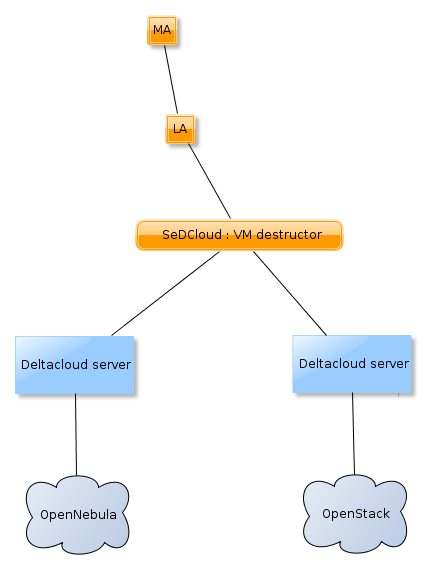
\includegraphics[width=0.7\textwidth]{fig/SeDCloudVMDestructor}
  \caption{VMs destructor over a federation of clouds}
  \label{fig:SeDCloudDestructor}
 \end{center}
\end{figure}


\begin{table}[h!]
\begin{tabular}{|c|c|c|p{0.5\textwidth}|} 
  \hline
  \multicolumn{4}{|c|}{Service name : \textbf{\texttt{vm\_destruction\_by\_ip}}} \\
  \hline
    IN/OUT & Position & Type & Description \\
    \hline
    \multirow{2}{*}{IN} & 0 & DIET\_FILE & A file containing the ip addresses of the VM to destroy\\
    \cline{2-4}
                        & 1 & DIET\_INT & If 0 then the ip addresses of the VMs are considered by Deltacloud as public ip, private ip otherwise\\
    \hline
\end{tabular}
\caption{DIET profile of the service ``vm\_destruction\_by\_ip''}
\label{tab:vm-destruction-by-ip}
\end{table}
